\documentclass{article}
\usepackage{fullpage}
\usepackage{graphicx}

\def\file#1{\texttt{#1}}
\def\bench#1{\texttt{#1}}
\def\code#1{\texttt{#1}}

\usepackage{caption}
\author{Aur\`ele Barri\`ere \& Benjamin Fasquelle}
\title{Practical Evaluation}
\date{March 24, 2017}

\begin{document}
\maketitle

Except for question 1.1 (on 5 nodes), these experiments were done on 15 nodes. The log files will be sent with the report.

It would have been better to have several measures for each experiments, so our conclusions

\section*{Question 1.1}
To evaluate the usefulness of speculation in a stressed environment, we run several jobs with the same configuration and the same data, the only change being the activation of the speculative execution.

In each job, we are going to stress one of the 5 nodes. In this purpose, we used a script to stress the disk (see in Annex [?]) on only one node.

We used the benchmark \bench{sort} with a block size of 128MB, a replication factor of 3 and 8 map/reduce slots.

In the first two runs, we disable the speculation (speculative execution in \file{mapred-site.xml}).
In the next two runs, we enable the speculation.

%to be continued

We used a data set of 20GB, with replication factor 3.

Some results are presented in the Table 1.

\begin{center}
\captionof{table}{Measurement}
\begin{tabular}{|c|c|c|}
\hline
\ & Without speculation & With speculation \\
\hline
Execution time & 5mins, 55sec & 6mins, 58sec \\
\hline
Number of speculatives copies & 0 & 4 \\
\hline
Average Map runtime & 3sec & 5sec \\
\hline
Maximum Map runtime & 5sec & 11sec \\
\hline
Average Reduce runtime & 1mins, 48sec & 2mins, 4sec \\
\hline
Maximum Reduce runtime & 2mins, 18sec & 2mins, 40sec \\
\hline
\end{tabular}
\end{center}



Speculative tasks have lower priority, thus we can see on Figure (\ref{spec_prio}) that they are executed at the end (tasks in red).

\begin{figure}%[h!]
  \centering
  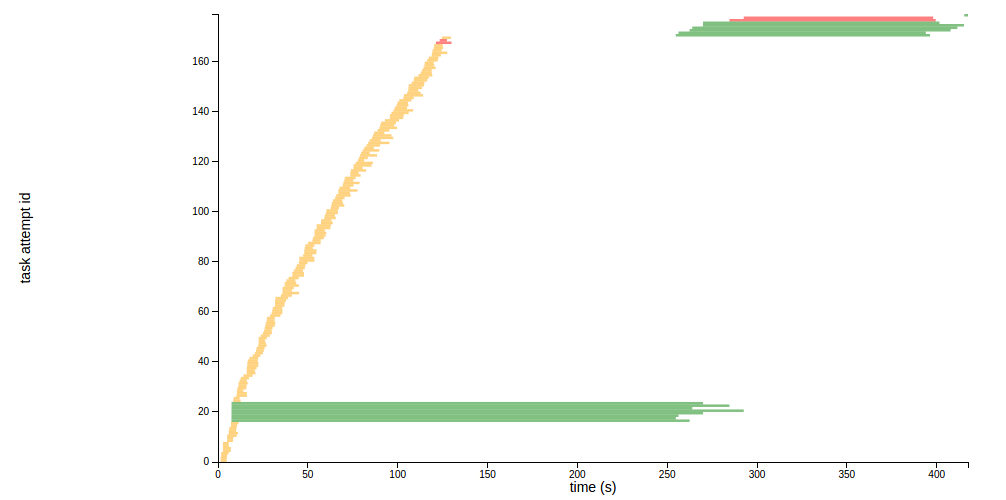
\includegraphics[width=0.6\textwidth]{spec.png}
  \caption{Executions of the tasks with speculation}
  \label{spec_prio}
\end{figure}


\section*{Question 1.2}

We used a data set of 20GB and run sort benchmark using block size at 128MB and the replication factor at 3.

We execute runs with different expiry interval (30seconds and 1 minutes), and stop the tasktracker daemon on one node (one time before the completion of the map tasks, another after this completion).

The next tables show the execution times and the number of killed tasks respectively.

\begin{center}
\captionof{table}{Execution times} 
\begin{tabular}{|c|c|c|}
\hline
\ & expiry interval: 30 seconds & expiry interval: 1 minute \\
\hline
Before completion map & 8mins, 58sec & 14mins, 3sec \\
\hline
After completion map & 14mins, 41sec & 12mins, 27sec\\
\hline
\end{tabular}
\end{center}

\begin{center}
\captionof{table}{Number of killed tasks} 
\begin{tabular}{|c|c|c|}
\hline
\ & expiry interval: 30 seconds & expiry interval: 1 minute \\
\hline
Before completion map & 4 & 11 \\
\hline
After completion map & 21 & 13 \\
\hline
\end{tabular}
\end{center}


\begin{figure}%[h!]
  \centering
  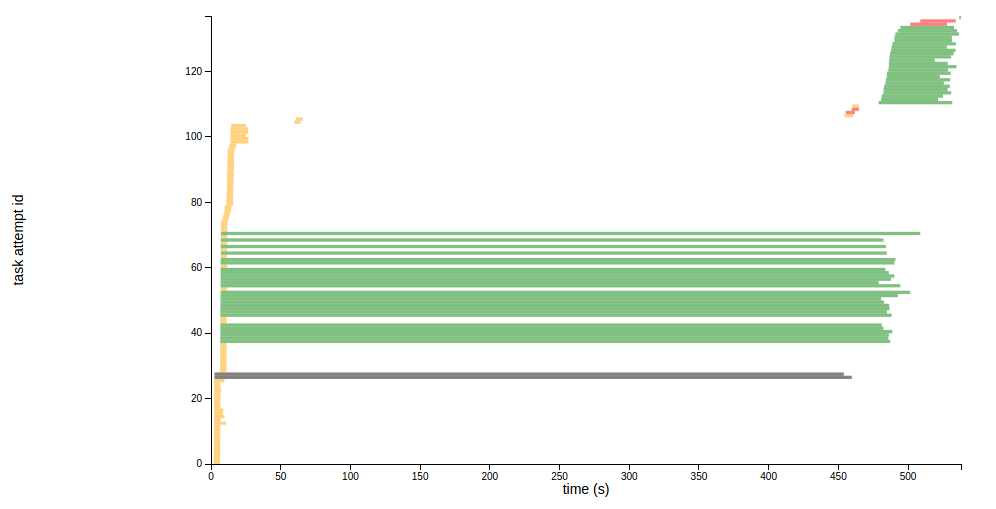
\includegraphics[width=0.4\textwidth]{expiry30before.png}
  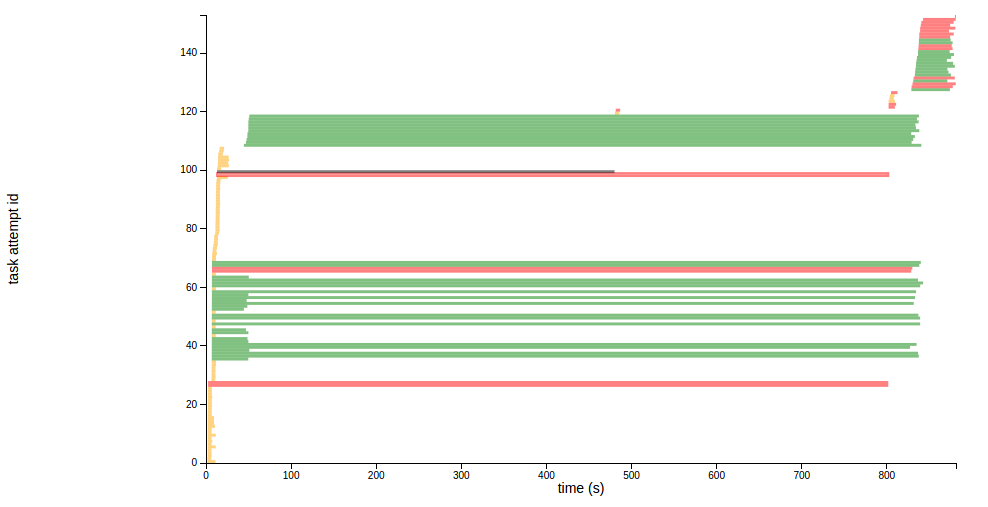
\includegraphics[width=0.4\textwidth]{expiry30after.png}
  \caption{Left: Tasktracker daemon stop before (left) and after (right) the completion of the map tasks (30sec)}
  \label{kill}
\end{figure}




I'm not really sure how to interpret this result.

\section*{Question 2.1}


We used a data set of 10GB and run wordcount and sort benchmarks using
different values (0.05, 0.5, and 1) of slowstart.
It means that the reduce phase will only start of some percentage of the map phase is done (5\%, 50\% or 100\%).

The next table shows the execution times.

\begin{center}
\captionof{table}{Execution times} 
\begin{tabular}{|c|c|c|}
\hline
\ & Sort & Wordcount \\
\hline
0.05 & 1mins, 2sec & 6mins, 55sec \\
\hline
0.5 & 1mins, 19sec & 6mins, 36sec \\
\hline
1 & 1mins, 7sec & 6mins, 52sec \\
\hline
\end{tabular}
\end{center}

For the sort benchmarks, we can see that the time taken by Map tasks is the same for all the values (3sec in average, 7 at worst).
However, the time taken by Shuffle decrease when the value increase: in average, it is 15sec for 0.05 (18 at worst), 12sec for 0.5 (17 at worst) and 11sec for 1 (14 at worst). For the time taken by Reduce tasks, it's more quickly with the value at 0.5: it is 7sec in average (11 at worst), against 11sec for 0.05 (17 at worst) and 10sec for 1 (14 at worst).
%We can observe that if we want to reduce the global execution time, we can increase the value, that is reduce the Shuffle time, but the Reduce time is lower for the value at 0.5.

For the Wordcount benchmarks, we can see the same thing for the Map time and the Shuffle time, but for the Reduce time, it decreases when the value of slowstart increases: on average, it is 4minutes and 26sec for 0.05 (4mins, 45sec at worst), 3minutes and 46sec for 0.05 (4mins, 15sec at worst) and 3minutes and 40sec for 1 (3mins, 59sec at worst).

In the Wordcount example, the reduce phase does not benefit from starting early, because the reduce nodes need data from all of the map and shuffle nodes. Launching reduce jobs too early might use some resource that wasn't needed. 


\begin{figure}%[h!]
  \centering
  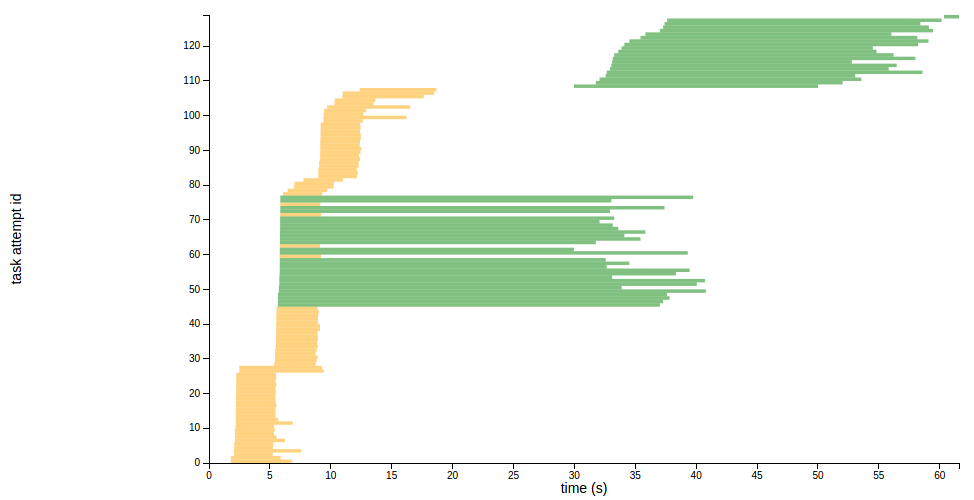
\includegraphics[width=0.4\textwidth]{sort005.png}
  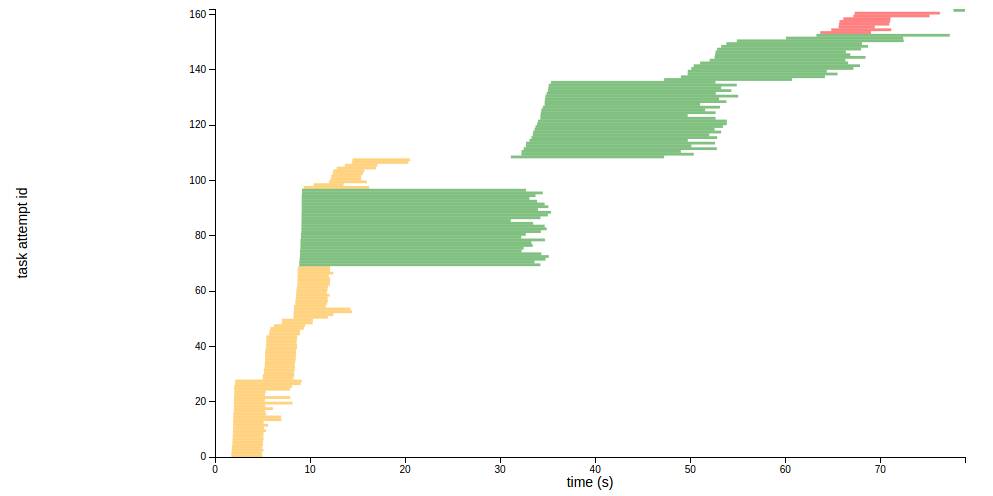
\includegraphics[width=0.4\textwidth]{sort05.png}
  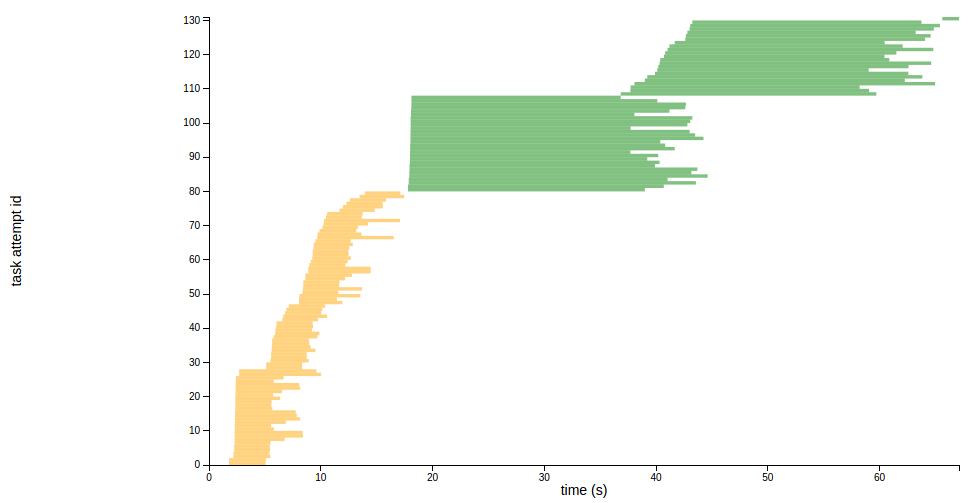
\includegraphics[width=0.4\textwidth]{sort1.png}
  \caption{Sort with value at 0.05 (left), 0.5 (right) and 1 (below)}
  \label{values}
\end{figure}

We can see on Figure (\ref{values}) that the start of the Reduce tasks rely on the value, as expected.



\section*{Question 3.1}


We run 6 sort applications on different sizes (3*2GB, 2*4GB 1*10GB) under Fifo scheduler, Fair scheduler (preemption disabled), and Fair scheduler
(preemption enabled) (we used Fair scheduler within the pool).

Jobs were launched with a decreasing input size order and 10 second interval between two
jobs.

%See the execution time, data locality and the waiting time of the applications. what can
%you observe?

The next table shows the execution times.

\begin{center}
\captionof{table}{Execution times} 
\begin{tabular}{|c|c|c|c|}
\hline
\ & Fifo & Fair & Fair with preemption \\
\hline
2GB & 36sec & 31sec & 31sec \\
\hline
2GB & 36sec & 30sec & 30sec \\
\hline
2GB & 38sec & 28sec & 31sec \\
\hline
4GB & 48sec & 46sec & 36sec \\
\hline
4GB & 53sec & 52sec & 37sec \\
\hline
10GB & 1mins, 17sec & 1mins, 13sec & 1mins, 11sec \\
\hline
\end{tabular}
\end{center}

Fair scheduler can be bad for data locality.

\begin{figure}%[h!]
  \centering
  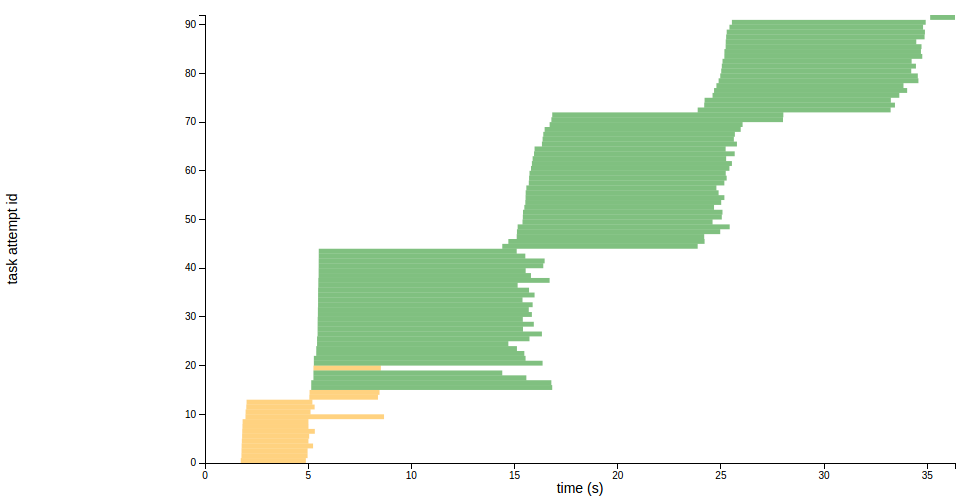
\includegraphics[width=0.4\textwidth]{fifo2.png}
  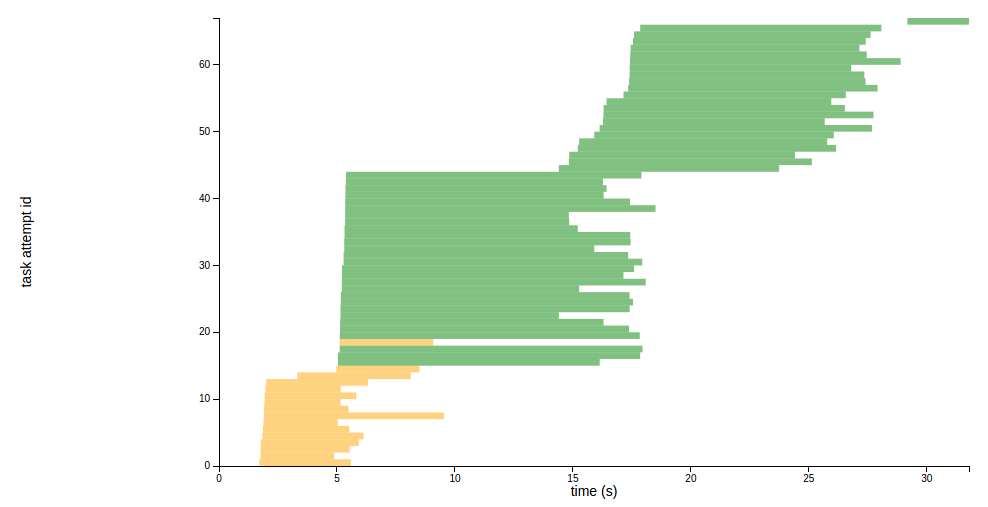
\includegraphics[width=0.4\textwidth]{fair2.png}
  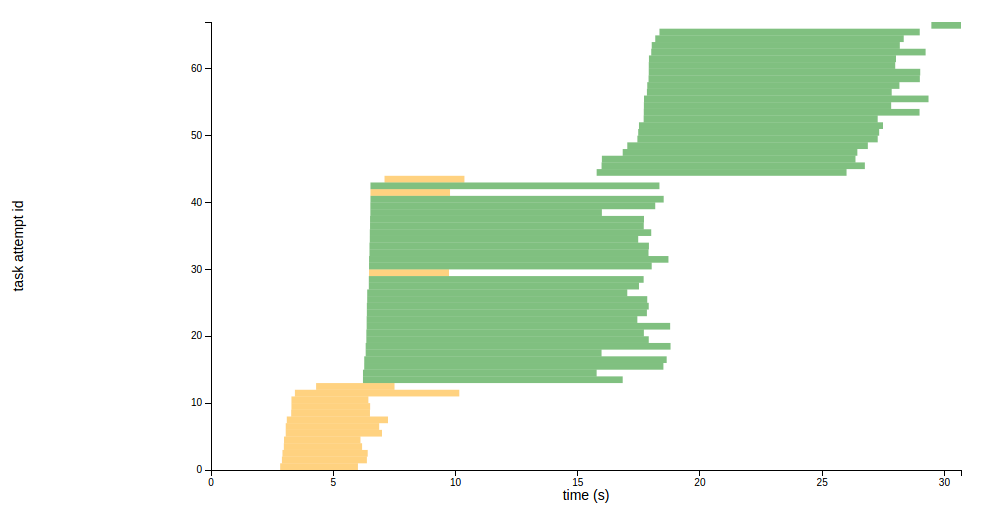
\includegraphics[width=0.4\textwidth]{fair_preemp2.png}
  \caption{Last sort applications with Fifo (left), Fair without preemption (right) and Fair with preemption (below)}
  \label{fair}
\end{figure}



\section*{Annex}
% put the script for disk stress


\end{document}
